\chapter{Resultados e Discussão}
\section{Organização das evidências}
Os resultados preliminares são separados por universo experimental. O controle de 375 imagens responde prioritariamente à questão sobre ângulo e distância. O acervo de 2.300 imagens fornece contexto para o YOLO11s original. O subconjunto de 380 imagens permite uma comparação observacional entre os dois detectores. Os denominadores desses conjuntos não são somados. No acervo observacional, o Faster R-CNN foi avaliado apenas no subconjunto de 380 imagens. As diferenças são descritivas, sem intervalos de confiança ou testes de significância nesta análise.

\section{Resultado principal: ângulo com distância controlada}
A Tabela \ref{tab:recall-celulas} contém todas as 15 combinações. O número de referências é 25 em cada linha para cada modelo. Os FN são obtidos por $25-VP$; as porcentagens são recall, não precisão.
\begin{table}[htb]
\caption{Recall e verdadeiros positivos no experimento controlado}
\label{tab:recall-celulas}\centering\small
\begin{tabular}{rr r r r r}
\hline Distância & Ângulo & VP YOLO & Recall YOLO & VP Faster & Recall Faster\\\hline
10 m & $0^\circ$ & 1 & 4\% & 9 & 36\%\\
10 m & $15^\circ$ & 6 & 24\% & 17 & 68\%\\
10 m & $30^\circ$ & 20 & 80\% & 24 & 96\%\\
10 m & $45^\circ$ & 25 & 100\% & 25 & 100\%\\
10 m & $60^\circ$ & 25 & 100\% & 25 & 100\%\\\hline
20 m & $0^\circ$ & 0 & 0\% & 0 & 0\%\\
20 m & $15^\circ$ & 0 & 0\% & 1 & 4\%\\
20 m & $30^\circ$ & 15 & 60\% & 11 & 44\%\\
20 m & $45^\circ$ & 21 & 84\% & 20 & 80\%\\
20 m & $60^\circ$ & 25 & 100\% & 23 & 92\%\\\hline
40 m & $0^\circ$ & 0 & 0\% & 0 & 0\%\\
40 m & $15^\circ$ & 0 & 0\% & 0 & 0\%\\
40 m & $30^\circ$ & 0 & 0\% & 0 & 0\%\\
40 m & $45^\circ$ & 3 & 12\% & 5 & 20\%\\
40 m & $60^\circ$ & 15 & 60\% & 17 & 68\%\\\hline
\end{tabular}
\source[Relatório consolidado de influência do ângulo, p. 27; somente pesos pré-treinados.]
\end{table}

\begin{figure}[htb]
\caption{Recall em função do off-nadir, separado por distância e detector pré-treinado}
\centering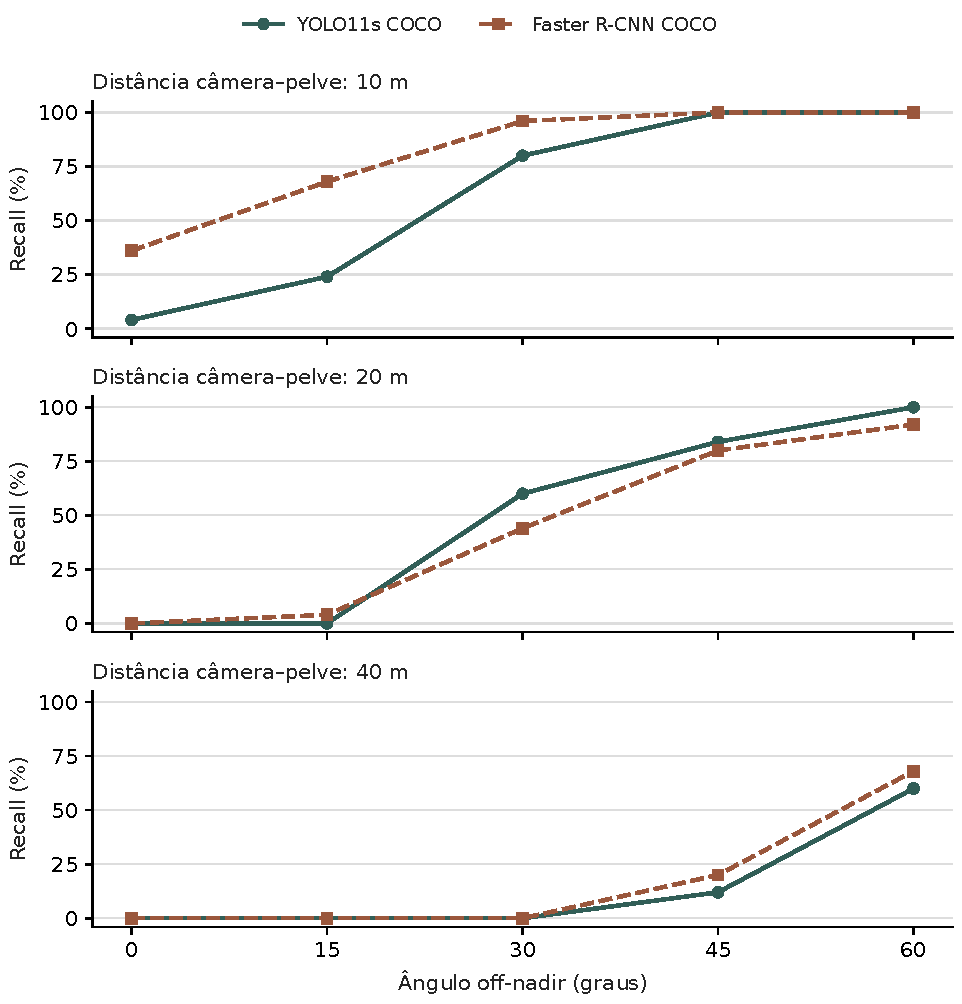
\includegraphics[width=\textwidth]{controle_recall_curvas.pdf}
\label{fig:recall-angular}
\source[Elaboração a partir da Tabela \ref{tab:recall-celulas}; 25 alvos por ponto.]
\end{figure}

Em 10 m, os dois modelos atingem 100\% de recall em $45^\circ$ e $60^\circ$. O Faster detecta mais alvos em $0^\circ$, $15^\circ$ e $30^\circ$. Em 20 m, o YOLO apresenta recall superior a partir de $30^\circ$, chegando a 100\% em $60^\circ$, contra 92\% do Faster. Em 40 m, ambos falham em todas as referências de $0^\circ$ a $30^\circ$, e o recall sobe para 60\% e 68\%, respectivamente, em $60^\circ$.

Dentro do intervalo e das condições avaliadas, o recall aumenta ou permanece estável com a obliquidade nos dois detectores. $60^\circ$ alcança o máximo em cada distância, empatando com $45^\circ$ em 10 m. Esse destaque é restrito ao intervalo estudado. Outros ângulos, azimutes, terrenos, poses e recursos visuais não foram avaliados, e o estudo não inclui imagens reais.

As curvas mudam com a distância: em $30^\circ$, por exemplo, o YOLO apresenta 80\%, 60\% e 0\% de recall a 10, 20 e 40 m. Esse padrão mostra que uma média angular única ocultaria condições importantes. A variação da silhueta projetada e a escala aparente são explicações plausíveis, não causas isoladamente comprovadas por esta análise. A Seção \ref{sec:objetos-pequenos} fundamenta a sensibilidade à escala e à localização das caixas, sem classificar automaticamente todas as referências de 40 m como pequenas. Embora a distância 3D seja fixa dentro de cada curva, a altura e a separação horizontal variam com o ângulo.

\subsection{Diferenças entre as condições de captura}
A comparação de $0^\circ$ com $60^\circ$ permite quantificar a amplitude observada em cada distância. No YOLO11s, o aumento de recall foi de 96 pontos percentuais em 10 m, 100 em 20 m e 60 em 40 m. No Faster R-CNN, os aumentos foram de 64, 92 e 68 pontos percentuais. São diferenças entre proporções no mesmo delineamento, e não ganhos relativos ou testes de significância.

Esse contraste não elimina a importância das condições intermediárias. Em 20 m, por exemplo, o YOLO apresenta recall maior que o Faster a partir de $30^\circ$, enquanto o Faster se destaca nas vistas de menor inclinação em 10 m. A comparação por célula impede que o agregado seja interpretado como domínio de um detector em todas as capturas.

O maior recall nas vistas oblíquas acompanha a direção descrita por \citeonline{lee2021synthetic}. Os modelos e as imagens diferem entre os estudos; a concordância é qualitativa e não comprova equivalência dos resultados.

\subsection{Exemplos de previsões nas capturas controladas}
A Figura \ref{fig:controle-previsoes} aproxima a leitura quantitativa do conteúdo das imagens. São seis registros do primeiro ator, nas duas inclinações extremas e nas três distâncias. As caixas já estavam presentes no relatório de execução do YOLO11s original: a referência aparece em verde e as propostas com confiança de pelo menos 0,25, em azul. A legenda VP ou FN descreve a recuperação da referência no ponto operacional; uma imagem marcada como FN ainda pode conter uma proposta sem pareamento, contabilizada como FP.

\begin{figure}[htb]
\caption{Exemplos do YOLO11s COCO: referência, previsão e omissão no controle}
\centering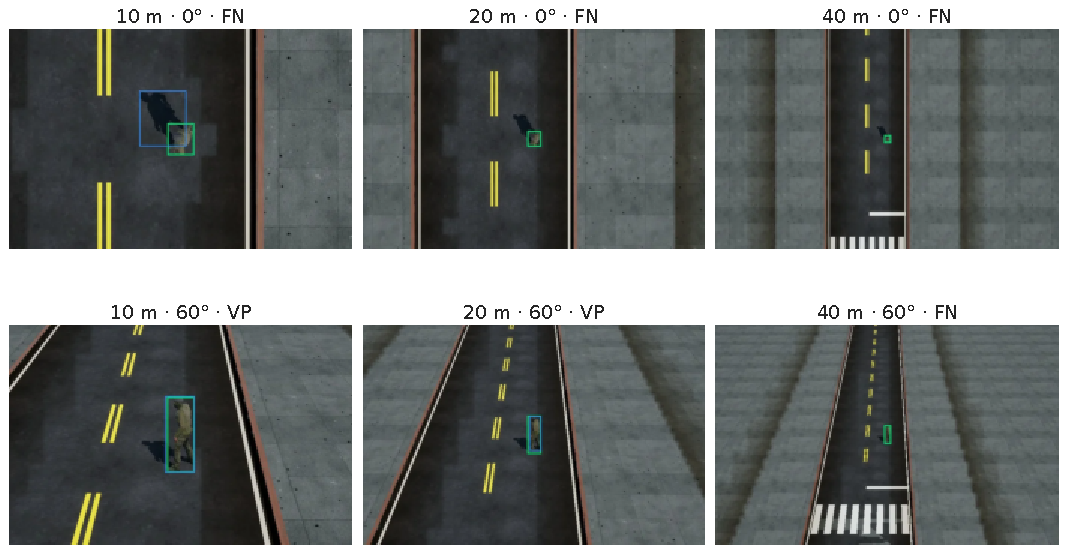
\includegraphics[width=\textwidth]{controle_exemplos_predicoes.pdf}
\label{fig:controle-previsoes}
\source[Recortes documentados no relatório do experimento controlado, p. 15--17, somente painel do modelo original; verde: referência; azul: proposta.]
\end{figure}

Em 10 m e $0^\circ$, existe uma caixa prevista, mas ela abrange sobretudo a sombra e não satisfaz o IoU mínimo com a referência do corpo. Esse caso ilustra a coexistência de FP e FN em uma mesma imagem: o sistema produz uma resposta sem localizar adequadamente o alvo elegível. Em 10 e 20 m a $60^\circ$, o mesmo ator é recuperado. Em 40 m a $60^\circ$, ele permanece sem pareamento no exemplo, apesar de essa célula apresentar 15 acertos entre os 25 atores no YOLO.

A última comparação mostra por que uma captura não representa todo o resultado de sua célula. O primeiro ator pode falhar em uma condição em que outros acertam, e um exemplo favorável também não comprova ausência de erros no conjunto. As imagens ilustram manifestações observáveis de acerto, omissão e localização inadequada, sem estimar a frequência de cada mecanismo visual no conjunto.
\FloatBarrier

\section{Qualidade global no controle}
\begin{table}[htb]
\caption{Contagens e qualidade de detecção nas 375 capturas controladas}
\label{tab:controle-global}\centering\small
\begin{tabular}{lrrrrrr}
\hline Modelo & VP & FP & FN & Precisão & Recall & F1\\\hline
YOLO11s & 156 & 69 & 219 & 69,33\% & 41,60\% & 52,00\%\\
Faster R-CNN & 177 & 95 & 198 & 65,07\% & 47,20\% & 54,71\%\\\hline
\end{tabular}
\source[Comparação Faster R-CNN, p. 1; confiança 0,25 e IoU 0,50.]
\end{table}

O Faster recupera 21 alvos a mais, mas produz 26 FP adicionais. Sua vantagem de recall é 5,60 pontos percentuais, e a de F1 é 2,71 pontos percentuais. O YOLO tem precisão 4,26 pontos percentuais superior. Não há um único vencedor para todos os critérios.

Os FP por distância são 58, 11 e 0 no YOLO e 74, 20 e 1 no Faster, respectivamente a 10, 20 e 40 m. Na célula de 10 m e $60^\circ$, ambos registram 25 VP, zero FP e zero FN. Uma caixa desenhada, por si só, não demonstra acerto: também deve satisfazer confiança, classe e correspondência com a referência elegível.

\begin{table}[htb]
\caption{AP calculado com avaliador COCO comum, em porcentagem}
\label{tab:ap-comum}\centering\small
\begin{tabular}{llrr}
\hline Conjunto & Modelo & $AP_{50}$ & $AP_{50:95}$\\\hline
Controlado (375) & YOLO11s & 49,59 & 40,70\\
Controlado (375) & Faster R-CNN & 50,94 & 39,82\\
Comparativo (380) & YOLO11s & 29,15 & 16,90\\
Comparativo (380) & Faster R-CNN & 27,66 & 14,62\\\hline
\end{tabular}
\source[Comparação Faster R-CNN, p. 15; COCOeval, maxDets=100.]
\end{table}

No controle, o Faster tem $AP_{50}$ ligeiramente maior, mas o YOLO apresenta $AP_{50:95}$ maior. AP agrega a ordenação dos escores e exigências de localização, por isso seu ordenamento pode divergir do recall a confiança fixa. Os antigos valores de AP provenientes do validador Ultralytics não são utilizados na Tabela \ref{tab:ap-comum}.

\begin{figure}[htb]
\caption{Comparação global dos detectores nas 375 imagens controladas}
\centering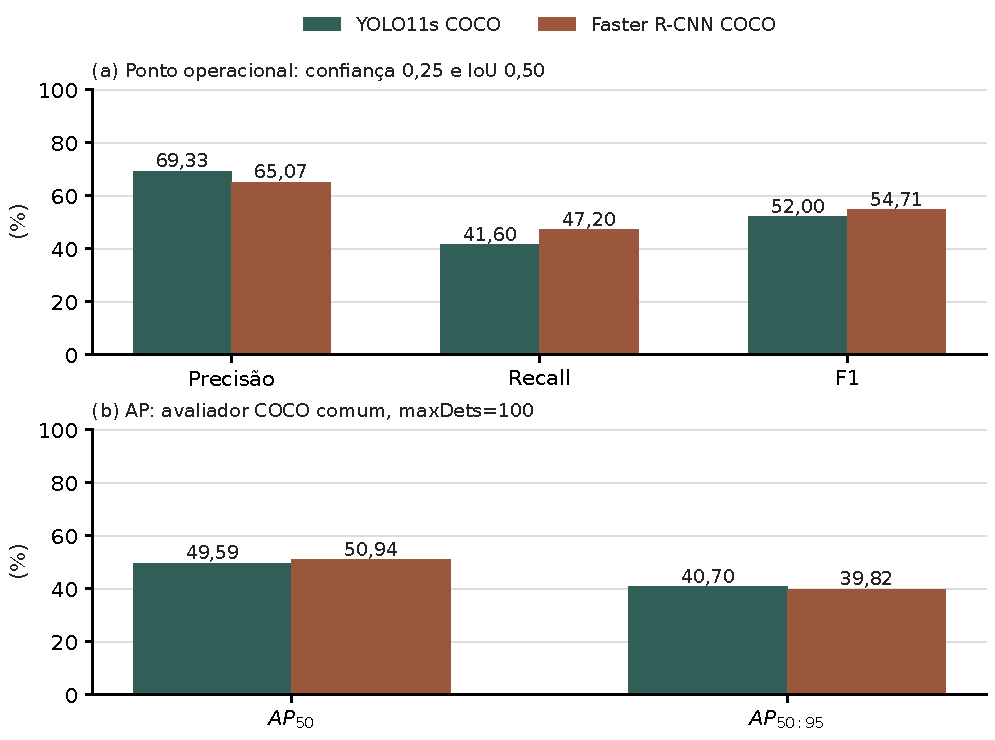
\includegraphics[width=\textwidth]{controle_metricas_globais.pdf}
\label{fig:controle-metricas}
\source[Elaboração a partir de resumo\_modelos.csv, selecionando os dois modelos originais; AP do avaliador COCO comum.]
\end{figure}

A Figura \ref{fig:controle-metricas} apresenta os mesmos agregados em dois painéis, pois precisão, recall e F1 se referem ao ponto operacional, enquanto AP considera a ordenação das propostas em diferentes escores. O painel superior torna visível a troca entre recuperar mais alvos e aceitar mais previsões incorretas. O inferior mostra que a ordem entre os modelos muda quando a localização é exigida em múltiplos limiares de IoU. As diferenças não constituem uma análise de significância e não sustentam a escolha de um detector universalmente superior.
\FloatBarrier

\section{Distribuição das omissões e dos falsos positivos no controle}
A Figura \ref{fig:controle-f1-fp} complementa as curvas de recall com F1 e FP em todas as quinze condições. Em cada linha, a distância é mantida; em cada coluna, o ângulo é comum aos dois detectores. As escalas de F1 e FP representam grandezas diferentes, mas são iguais entre modelos para a mesma medida. F1 reúne precisão e recall, enquanto os FP permanecem apresentados como contagem absoluta.

\begin{figure}[htb]
\caption{F1 e falsos positivos por ângulo, distância e detector no controle}
\centering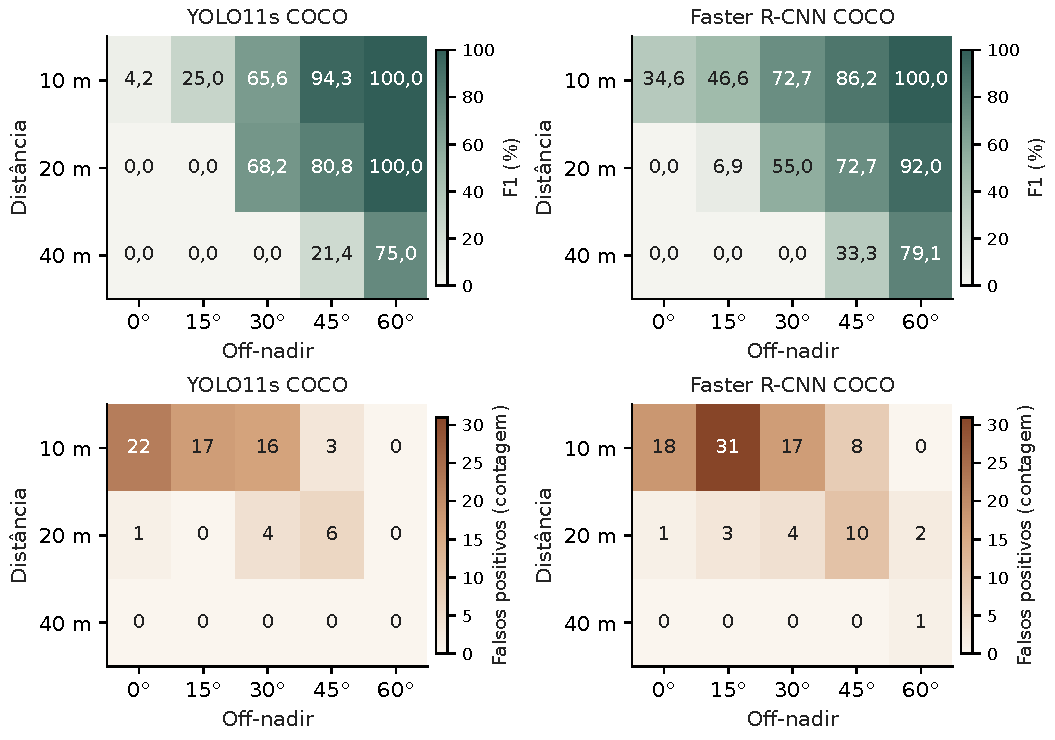
\includegraphics[width=\textwidth]{controle_f1_fp_celulas.pdf}
\label{fig:controle-f1-fp}
\source[Elaboração a partir de controlado\_celulas.csv; 25 referências por célula, confiança 0,25 e IoU 0,50.]
\end{figure}

Em 10 m, o aumento do recall entre $30^\circ$ e $60^\circ$ acompanha a redução de FP: de 16 para zero no YOLO e de 17 para zero no Faster. Em $45^\circ$, ambos recuperam todos os alvos, mas o YOLO ainda registra três FP e o Faster, oito. Por isso, seus F1 são aproximadamente 94,3\% e 86,2\%, apesar do recall de 100\% nos dois. Apenas em $60^\circ$, nessa distância, os dois combinam 25 VP, nenhum FN e nenhum FP.

O Faster produz 31 FP em 10 m e $15^\circ$, mesmo havendo apenas 25 pessoas de referência nessa célula. Isso é possível porque uma imagem pode gerar várias previsões sem correspondência; a contagem de FP não é limitada pelo número de alvos. Sem examinar cada proposta, não é possível distribuir esse total entre duplicatas, fundo e localização inadequada.

Em 40 m e $45^\circ$, os dois modelos têm precisão de 100\%, pois suas poucas propostas válidas são acertos: três no YOLO e cinco no Faster, sem FP. Entretanto, restam 22 e 20 FN. Os recalls são apenas 12\% e 20\%, e os F1, 21,4\% e 33,3\%. Esse caso mostra que alta precisão com poucas respostas não caracteriza recuperação satisfatória das pessoas. Nas células sem nenhuma previsão, a precisão é indefinida; o gráfico não a substitui artificialmente por 100\%.
\FloatBarrier

\subsection{O que a agregação por distância mostra e o que ela esconde}
Na Figura \ref{fig:controle-contagens}, cada distância reúne os cinco ângulos e contém 125 referências. A parte sólida das barras representa VP, e a parte hachurada, FN. Os FP ficam em um painel separado: eles são previsões sem correspondência, não pessoas adicionais a serem somadas ao denominador de 125.

\begin{figure}[htb]
\caption{Referências recuperadas, omissões e falsos positivos por distância no controle}
\centering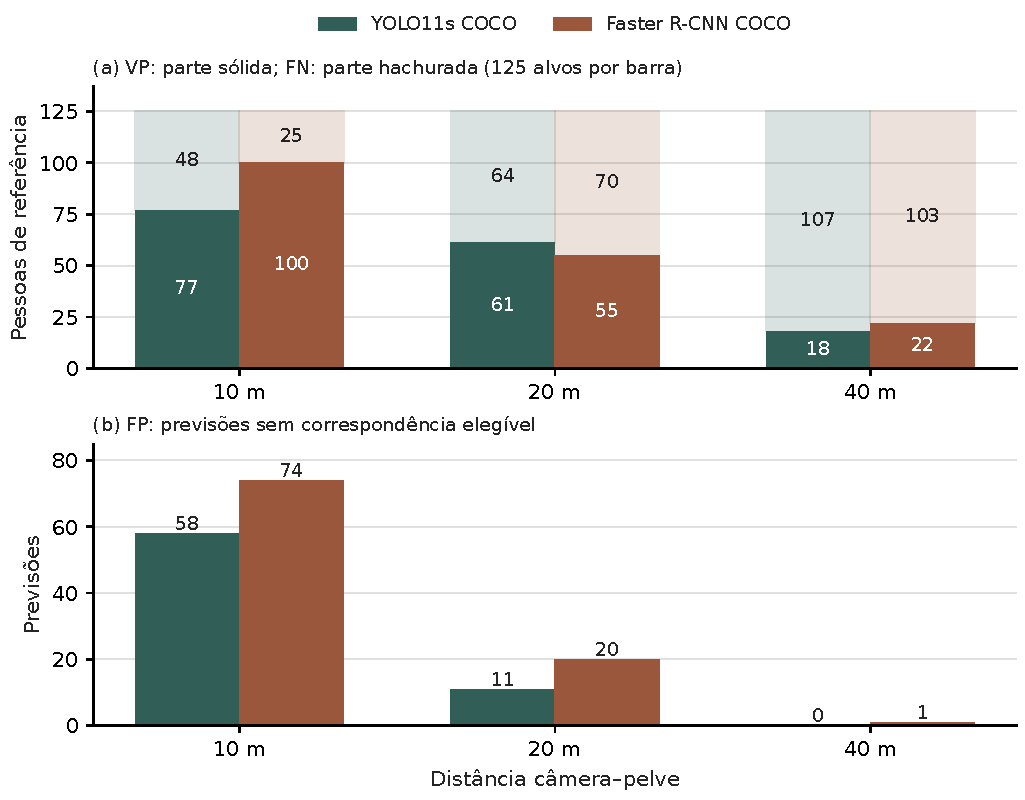
\includegraphics[width=\textwidth]{controle_contagens_distancia.pdf}
\label{fig:controle-contagens}
\source[Contagens somadas de controlado\_celulas.csv; cinco ângulos e 125 referências em cada distância, para cada detector.]
\end{figure}

Em 10 m, o YOLO recupera 77 das 125 referências, contra 100 no Faster. Em 20 m, a ordem se inverte: são 61 e 55 acertos. Em 40 m, os totais caem para 18 e 22. A quantidade de omissões nessa última distância é, portanto, 107 no YOLO e 103 no Faster. Esses totais não invalidam os acertos em $60^\circ$; mostram que as demais inclinações continuam difíceis e reduzem a recuperação quando os cinco ângulos são reunidos.

Os FP se concentram em 10 m e se tornam raros em 40 m, mas essa queda coexiste com muitas omissões. Assim, não se interpreta a ausência de FP em uma distância como melhora isolada do detector. Da mesma forma, a queda agregada de recall com a distância é descritiva deste conjunto balanceado: ela não identifica, sozinha, quanto da falha decorre de escala, silhueta ou outra característica da imagem.

Em conjunto, os gráficos respondem a perguntas distintas. As curvas localizam a mudança de recall com o ângulo; a matriz de F1 e FP revela o custo das respostas em cada condição; as barras por distância mostram onde se acumulam omissões. A conclusão sobre captura deve preservar essas três leituras, pois a média global oculta tanto condições favoráveis quanto células sem qualquer acerto.
\FloatBarrier

\section{Contexto observacional: avaliação completa do YOLO11s}
\begin{table}[htb]
\caption{Resultados observacionais por cenário, somente YOLO11s pré-treinado}
\label{tab:observacional}\centering\small
\begin{tabular}{lrrrrrr}
\hline Cenário & VP & FP & FN & Precisão & Recall & F1\\\hline
Urban\_Centered\_1m & 2.088 & 441 & 10.412 & 82,56\% & 16,70\% & 27,79\%\\
Urban\_Spread & 2.512 & 275 & 3.847 & 90,13\% & 39,50\% & 54,93\%\\
Forest\_Centered\_50 & 1.177 & 400 & 13.560 & 74,64\% & 7,99\% & 14,43\%\\
Forest\_Spread & 0 & 3 & 2.754 & 0,00\% & 0,00\% & 0,00\%\\
Forest\_Low\_Altitude & 39 & 31 & 1.621 & 55,71\% & 2,35\% & 4,51\%\\\hline
Total & 5.816 & 1.150 & 32.194 & 83,49\% & 15,30\% & 25,86\%\\\hline
\end{tabular}
\source[Avaliação completa YOLO11s original, p. 1.]
\end{table}

A precisão global de 83,49\% coexiste com recall de apenas 15,30\%. A maior parte das referências elegíveis não é recuperada, e a precisão isolada seria uma síntese insuficiente. Urban\_Spread tem o maior recall entre os cenários; Forest\_Spread não apresenta acertos, apesar de conter 2.754 referências elegíveis. Isso não comprova que vegetação seja a causa exclusiva: distância, escala, enquadramento e visibilidade também variam.

\begin{figure}[htb]
\caption{Exemplo de captura do cenário urbano presente no registro técnico}
\centering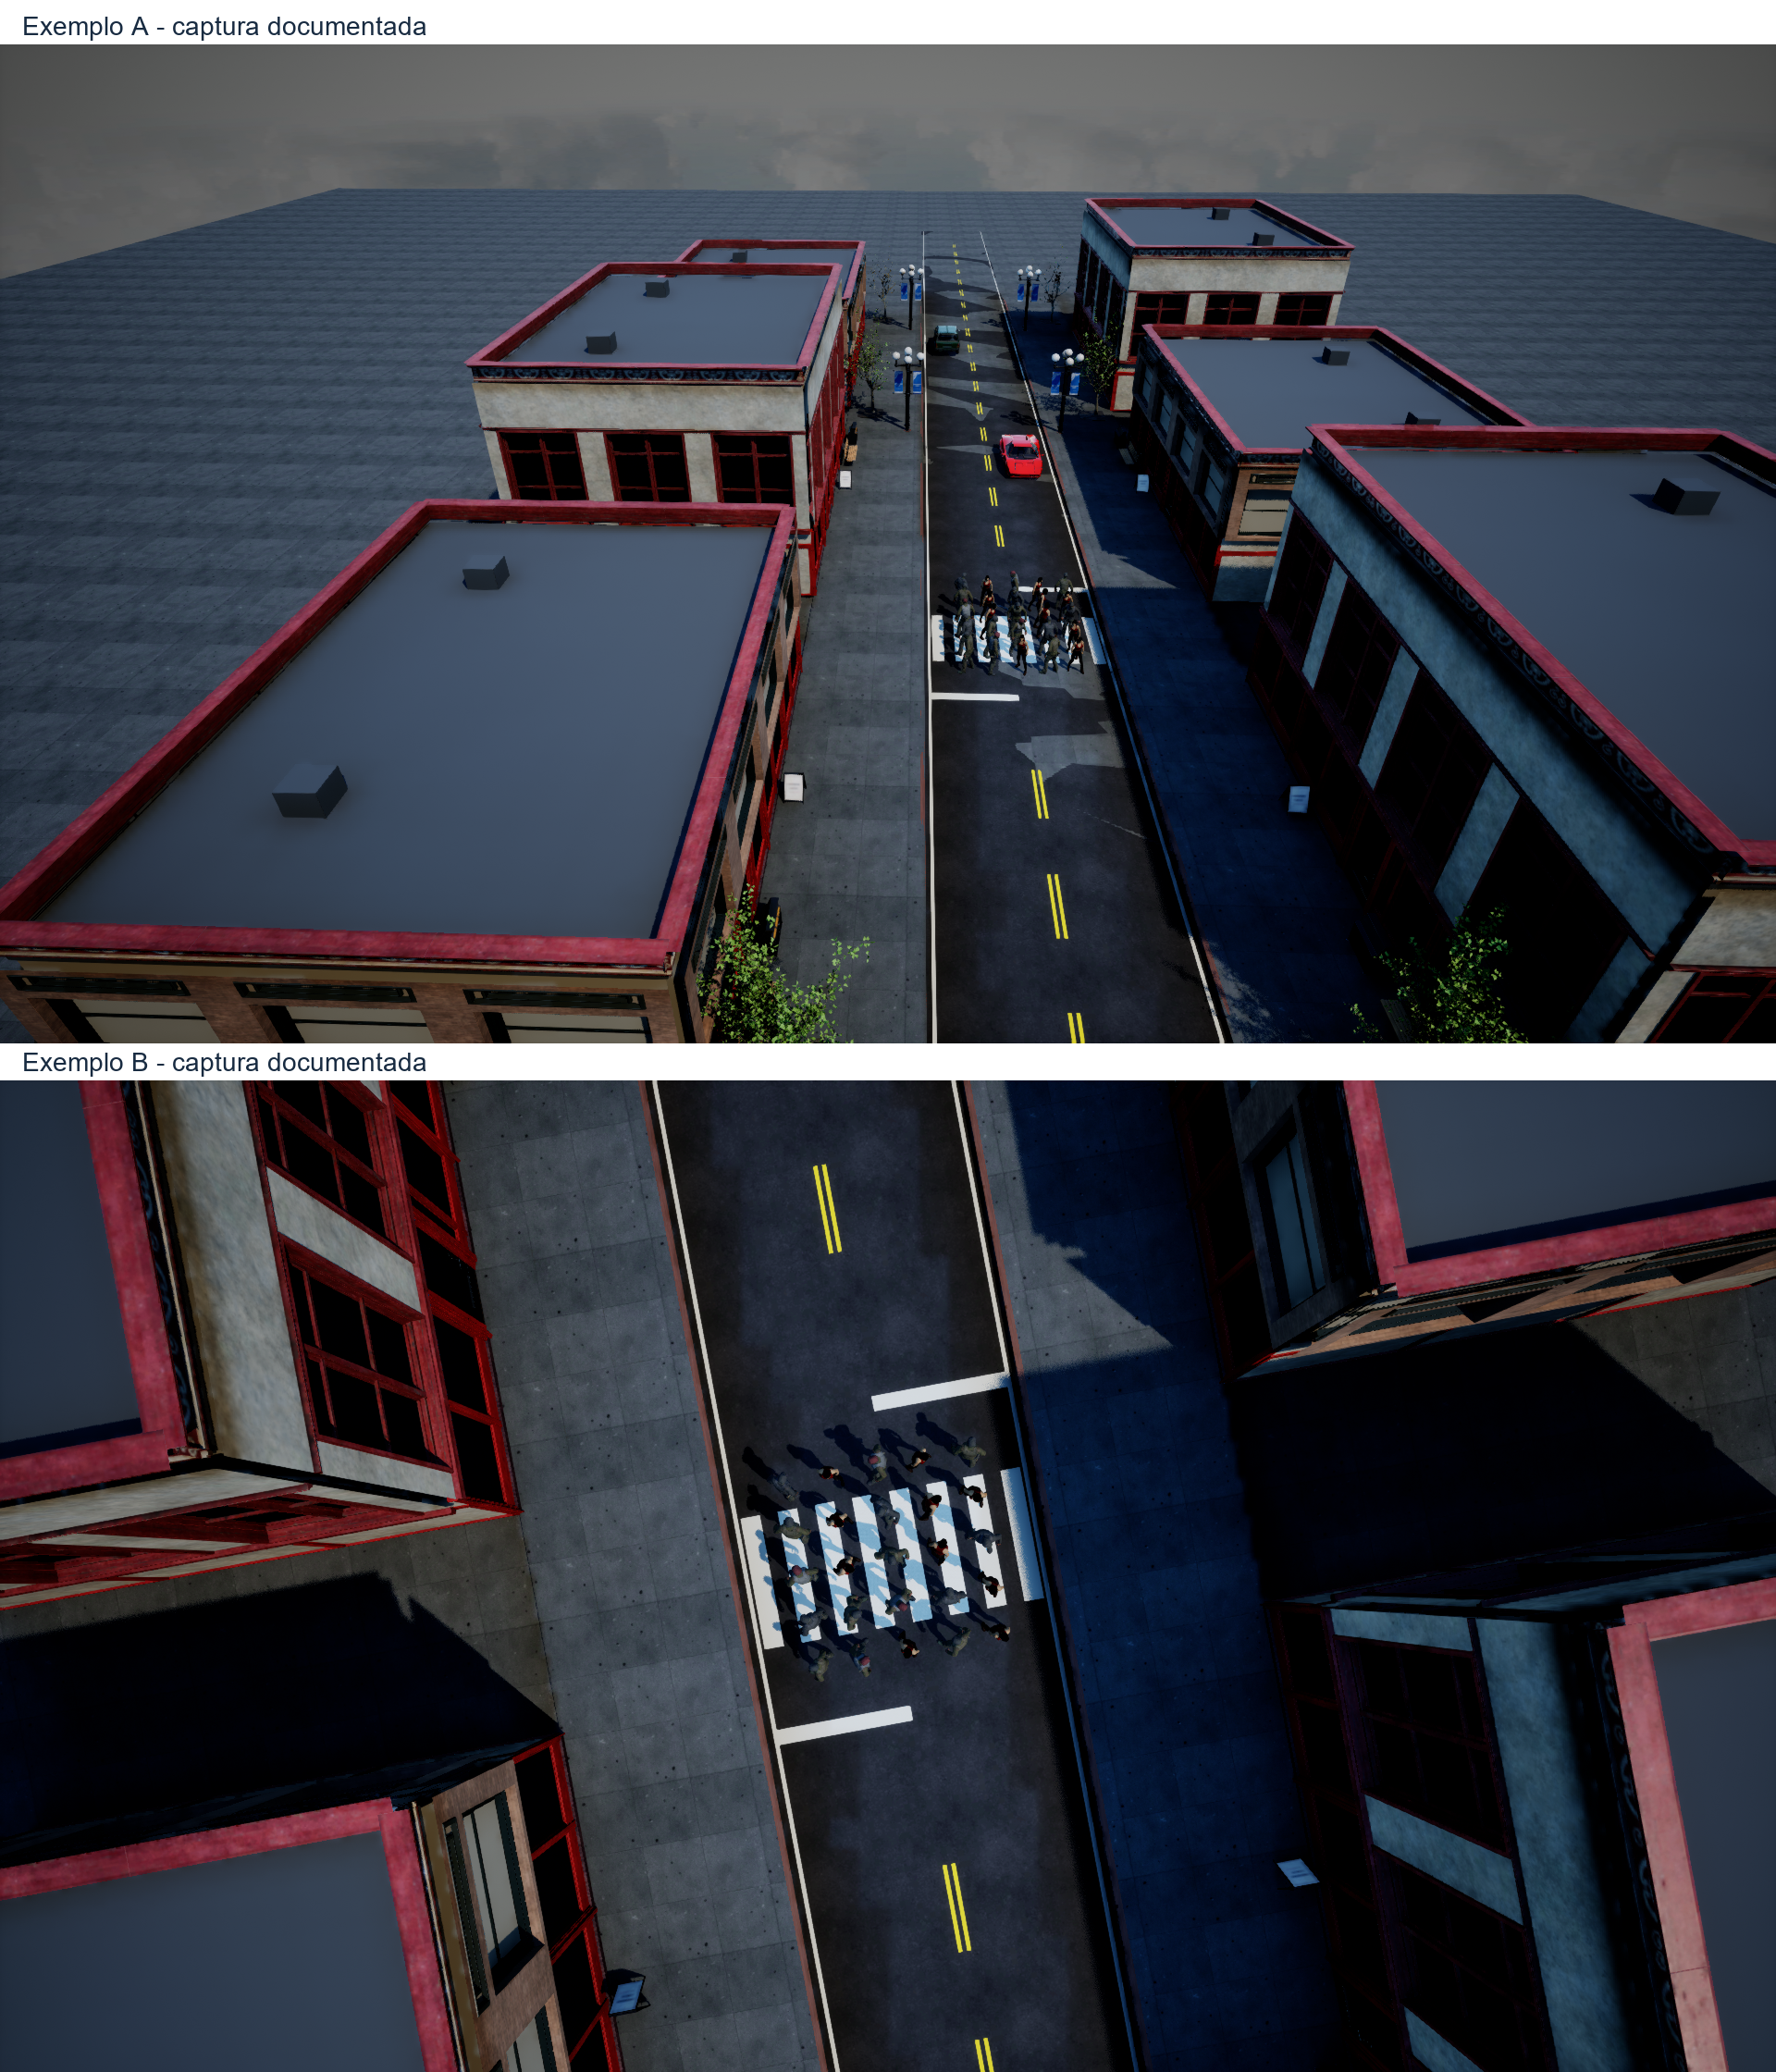
\includegraphics[width=0.94\textwidth]{exemplo_urbano_documentado.png}
\label{fig:urbano}
\source[Imagem extraída do registro Urban\_Centered\_1m, p. 5; exemplo de contexto, não nova medição.]
\end{figure}

O controle não substitui a dificuldade dos cenários completos. Ao retirar oclusores e manter um alvo visível, ele responde a uma pergunta mais delimitada. O aumento do recall agregado no controle não pode ser atribuído somente ao ângulo, pois o universo e a composição das imagens mudaram.

\subsection{Papel dos cinco mapas na análise complementar}
Os mapas observacionais não representam cinco repetições de um mesmo experimento controlado. O urbano centrado concentra os personagens em uma grade, enquanto o espalhado os distribui ao longo da avenida. Os três mapas florestais acrescentam vegetação e outras condições de visibilidade e captura. Essas configurações permitem identificar cenários de falha, mas não atribuir suas diferenças a um fator isolado.

O nome floresta de baixa altitude descreve uma configuração do acervo. Ele não garante, por si só, menor distância câmera--pelve para todas as pessoas ou maior quantidade de pixels visíveis do corpo. AGL, deslocamento horizontal, enquadramento e oclusão precisam ser examinados nos registros de cada relação pessoa--imagem.

Na floresta espalhada, apenas 2.754 das 15.000 relações são elegíveis. Na configuração de baixa altitude, são 1.660. Isso corresponde a aproximadamente 18,36\% e 11,07\% das relações de origem. Os recalls de 0\% e 2,35\% referem-se às referências que permaneceram elegíveis; eles não usam todas as relações do cenário como denominador. A distinção é necessária para interpretar os resultados e o alcance das exclusões.

Um recall muito baixo não torna o cenário cientificamente inútil. Com referências corretas e protocolo aplicado de forma consistente, ele documenta uma condição em que o sistema deixa de recuperar pessoas. O procedimento adequado é verificar os dados e investigar os erros, mantendo o resultado desfavorável quando ele for válido. Excluir mapas somente para elevar as métricas removeria uma parte relevante da evidência.

\subsection{Comparação angular com faixas de distância comuns}
Para reduzir diferenças de composição entre ângulos, o relatório do YOLO11s apresenta uma análise com faixas de distância presentes nos cinco ângulos de cada mapa. A seleção exige pelo menos vinte referências elegíveis por faixa e ângulo e utiliza os mesmos pesos entre ângulos. A Tabela \ref{tab:angular-observacional} conserva esse recorte; suas porcentagens não substituem os resultados agregados da Tabela \ref{tab:observacional}.

\begin{table}[htb]
\caption{Recall do YOLO11s por ângulo com padronização de distância, em porcentagem}
\label{tab:angular-observacional}\centering\small
\begin{tabular}{lrrrrrl}
\toprule Cenário & $0^\circ$ & $15^\circ$ & $30^\circ$ & $45^\circ$ & $60^\circ$ & Faixas\\\midrule
Urbano espalhado & 4,42 & 15,32 & 38,33 & 67,03 & 77,88 & D02--D04\\
Urbano centrado & 0,68 & 4,21 & 23,02 & 26,93 & 32,08 & D02--D04\\
Floresta centrada & 0,30 & 2,92 & 9,17 & 17,44 & 27,56 & D02--D04\\
Floresta baixa altitude & 0,00 & 0,29 & 1,05 & 2,08 & 5,93 & D03--D05\\
Floresta espalhada & 0,00 & 0,00 & 0,00 & 0,00 & 0,00 & D05\\\bottomrule
\end{tabular}
\source[Avaliação completa YOLO11s original, p. 10 e 20.]
\end{table}

Em quatro mapas, $0^\circ$ tem o menor recall e $60^\circ$ o maior. A floresta espalhada permanece sem acertos. O resultado acompanha a direção geral do controle, mas a padronização não fixa as pessoas visíveis, as oclusões ou os enquadramentos. Além disso, o eixo óptico não coincide com todas as linhas de visada em imagens com várias pessoas. Trata-se de evidência complementar, não de uma segunda intervenção controlada sobre o mesmo alvo.

As métricas marginais, sem a padronização, podem produzir outra ordenação entre ângulos. No urbano centrado, o relatório registra recall de 25,16\% em $45^\circ$ e 22,12\% em $60^\circ$; na floresta centrada, 14,45\% e 13,57\%, respectivamente. A mudança mostra por que a distribuição de distâncias precisa acompanhar a interpretação de uma curva angular.

\section{Comparação no subconjunto observacional}
\begin{table}[htb]
\caption{Comparação dos detectores em 380 imagens e 6.310 referências elegíveis}
\label{tab:subconjunto}\centering\small
\begin{tabular}{lrrrrrr}
\hline Modelo & VP & FP & FN & Precisão & Recall & F1\\\hline
YOLO11s & 1.071 & 174 & 5.239 & 86,02\% & 16,97\% & 28,35\%\\
Faster R-CNN & 1.761 & 1.640 & 4.549 & 51,78\% & 27,91\% & 36,27\%\\\hline
\end{tabular}
\source[Comparação Faster R-CNN, p. 1; mesmos arquivos e referências.]
\end{table}

O Faster apresenta 690 VP adicionais e 1.466 FP adicionais. Seu recall cresce 10,94 pontos percentuais em relação ao YOLO, enquanto a precisão é 34,24 pontos percentuais menor. Esses dados não identificam automaticamente quais objetos causaram os FP. Para separar fundo, duplicatas e caixas mal localizadas, é necessária inspeção das previsões.

No mesmo subconjunto, o recall por faixa de distância do YOLO é 23,61\%, 35,85\%, 15,37\%, 12,39\% e 5,83\%, enquanto no Faster é 50,82\%, 50,24\%, 29,71\%, 19,64\% e 13,10\%. Os denominadores são 305, 1.230, 1.178, 2.551 e 1.046 referências, respectivamente nas faixas definidas na metodologia. A faixa mais próxima não possui necessariamente maior recall, mostrando que distância isolada não resume os fatores presentes no acervo observacional.

\section{Custo computacional observado}
\begin{table}[htb]
\caption{Tempo por imagem em CPU: medições de escopo não equivalente}
\label{tab:tempo}\centering\small
\begin{tabular}{llrrr}
\hline Conjunto & Modelo & Média (s) & Mediana (s) & P95 (s)\\\hline
Comparativo & YOLO11s & 0,268 & 0,267 & 0,285\\
Comparativo & Faster R-CNN & 2,626 & 2,614 & 2,767\\
Controlado & YOLO11s & 0,268 & 0,268 & 0,279\\
Controlado & Faster R-CNN & 2,633 & 2,616 & 2,759\\\hline
\end{tabular}
\source[Comparação Faster R-CNN, p. 16; lote 1, sem benchmark temporal comum.]
\end{table}

Os registros sugerem custos operacionais distintos, porém o intervalo cronometrado não é equivalente. Não se publica uma razão rigorosa de velocidade nem FPS de um sistema completo. Eficiência temporal é análise complementar; a questão central permanece a detecção em função da geometria.

\section{Reprodutibilidade e rastreabilidade}
Repetir a análise exige conhecer a identidade dos arquivos e o protocolo que transforma previsões em métricas. Os registros consultados conservam identificadores de cenário, imagem e modelo, além de caixas, escores e resultados de pareamento. Essa estrutura permite consultar uma célula agregada e retornar às observações que a compõem.

O recálculo a partir de propostas salvas responde se as mesmas entradas e regras produzem as mesmas contagens. A repetição da inferência acrescenta a execução dos detectores e depende dos pesos e bibliotecas. Já uma nova captura exige o projeto Unreal completo e seu estado de cena. Esses procedimentos não são equivalentes, e a disponibilidade do PDF de resultados não substitui os arquivos necessários a cada um deles.

